\documentclass[addpoints,spanish, 12pt,a4paper]{exam}
%\documentclass[answers, spanish, 12pt,a4paper]{exam}
\printanswers
\pointpoints{punto}{puntos}
\hpword{Puntos:}
\vpword{Puntos:}
\htword{Total}
\vtword{Total}
\hsword{Resultado:}
\hqword{Ejercicio:}
\vqword{Ejercicio:}

\usepackage[utf8]{inputenc}
\usepackage[spanish]{babel}
\usepackage{eurosym}
%\usepackage[spanish,es-lcroman, es-tabla, es-noshorthands]{babel}


\usepackage[margin=1in]{geometry}
\usepackage{amsmath,amssymb}
\usepackage{multicol}
\usepackage{yhmath}

\pointsinrightmargin % Para poner las puntuaciones a la derecha. Se puede cambiar. Si se comenta, sale a la izquierda.
\extrawidth{-2.4cm} %Un poquito más de margen por si ponemos textos largos.
\marginpointname{ \emph{\points}}

\usepackage{graphicx}
\graphicspath{{../img/}} 

\newcommand{\class}{1º Bachillerato CCSS}
\newcommand{\examdate}{\today}
\newcommand{\examnum}{Examen final 2ª Evaluación}
\newcommand{\tipo}{A}


\newcommand{\timelimit}{80 minutos}

\renewcommand{\solutiontitle}{\noindent\textbf{Solución:}\enspace}


\pagestyle{head}
\firstpageheader{
\includegraphics[width=0.2\columnwidth]{header_left}}{\textbf{Departamento de Matemáticas\linebreak \class}\linebreak \examnum}{
\includegraphics[width=0.1\columnwidth]{header_right}}
\runningheader{\class}{\examnum}{Página \thepage\ of \numpages}
\runningheadrule


\begin{document}

\noindent
\begin{tabular*}{\textwidth}{l @{\extracolsep{\fill}} r @{\extracolsep{6pt}} }
\textbf{Nombre:} \makebox[3.5in]{\hrulefill} & \textbf{Fecha:}\makebox[1in]{\hrulefill} \\
 & \\
\textbf{Tiempo: \timelimit} & Tipo: \tipo 
\end{tabular*}
\rule[2ex]{\textwidth}{2pt}
Esta prueba tiene \numquestions\ ejercicios. La puntuación máxima es de \numpoints. 
La nota final de la prueba será la parte proporcional de la puntuación obtenida sobre la puntuación máxima. 

\begin{center}


\addpoints
 %\gradetable[h][questions]
	\pointtable[h][questions]
\end{center}

\noindent
\rule[2ex]{\textwidth}{2pt}

\begin{questions}
\question Una oficina bancaria ha tabulado las cantidades de dinero que retiran de sus cuentas 100 clientes jóvenes en
un determinado día:



\begin{tabular}{rlr}
\hline
    & Euros                  &   Clientes \\
\hline
  0 & $\left[0, 40\right)$   &         40 \\
  1 & $\left[40, 80\right)$  &         35 \\
  2 & $\left[80, 120\right)$ &         25 \\
\hline
\end{tabular}

\begin{parts}
\part[1] Realizar una tabla de frecuencias con los datos que vayas a necesitar para resolver el ejercicio

\begin{solution}\\

\begin{tabular}{rrrrrrrrrr}
\hline
    &   lim\_inf &   lim\_sup &   x\_i &   f\_i &   F\_i &   h\_i &    H\_i &   x\_if\_i &   x\^{}2\_if\_i \\
\hline
  0 &         0 &        40 &    20 &    40 &    40 &  0.4  &   0.4  &      800 &      16000 \\
  1 &        40 &        80 &    60 &    35 &    75 &  0.35 &   0.75 &     2100 &     126000 \\
  2 &        80 &       120 &   100 &    25 &   100 &  0.25 &   1    &     2500 &     250000 \\
  3 &       nan &       nan &   nan &   100 &   nan &  1    & nan    &     5400 &     392000 \\
\hline
\end{tabular}

\end{solution}
\part[1] Calcula la media y la varianza.
\begin{solution}
\{'media': 54.0, 'varianza': 1004.0, 'desviación típica': 31.6859590355097\}
\end{solution}
\part[1] Indica razonadamente en qué intervalos se encuentra la moda y la mediana respectivamente. 
\begin{solution}
\end{solution}
\part[2] Calcula la mediana. Ayuda:
$$P_k=L_i + \frac{k\frac{N}{100}-F_{i-1}}{f_i}\cdot C_i$$
\begin{solution}
 ${'k': 50, 'N': 100.0, 'L_i': 40.0, 'f_i': 35.0, 'F_{i-1}': 40.0, 'C_i': 40.0}$
 \\
 51.42857142857143
\end{solution}
\part[1] ¿Qué porcentaje de clientes ha retirado menos de 60\euro?
\begin{solution}
${'valor': 60, 'N': 100.0, 'L_i': 40.0, 'f_i': 35.0, 'F_{i-1}': 40.0, 'C_i': 40.0}$\\
57.5
\end{solution}

\end{parts}
\question La temperatura media en los meses de invierno en varias ciudades y el gasto medio por habitante en
calefacción ha sido:\\
\begin{tabular}{|c||c|c|c|c|c|c|}
\hline 
Temperatura (ºC) & 10 & 12 & 14 & 16  \\ 
\hline 
Gasto (\euro ) & 150 & 120 & 102 & 90  \\ 
\hline 
\end{tabular} 
\addpoints % to omit double points count

\begin{parts}
\part[1] ¿Cuál es el gasto medio?

\begin{solution}\\
\begin{tabular}{rrrrrr}
\hline
    &   x &     y &   xy &   x2 &    y2 \\
\hline
  0 &  10 & 150   & 1500 &  100 & 22500 \\
  1 &  12 & 120   & 1440 &  144 & 14400 \\
  2 &  14 & 102   & 1428 &  196 & 10404 \\
  3 &  16 &  90   & 1440 &  256 &  8100 \\
  \hline
  4 &  52 & 462   & 5808 &  696 & 55404 \\
  \hline
  5 &  13 & 115.5 & 1452 &  174 & 13851 \\
\hline
\end{tabular}
Gasto medio = 115.5
\end{solution}
\part[2] Halla el coeficiente de correlación lineal e interprétalo
\begin{solution}
covarianza	-49.5 \\
desvx	2.23606797749979 \\
desvy	22.599778759979046 \\
coefcorr -0.9795260923726159 \\
\end{solution}
\part[1] Estima el gasto medio por habitante de una ciudad si la temperatura media hubiera sido de 11ºC 

\begin{solution}
$y = -9.9x + 244.2$ \\
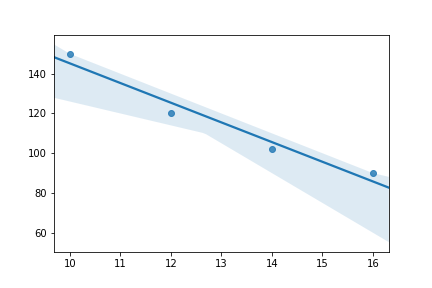
\includegraphics[scale=.5]{regresion1.png} \\
Valor estimado para 11: 135.3 \euro 

\end{solution}


\end{parts}



\question Calcula:
%\noaddpoints % to omit double points count

\begin{parts}
\part[1] $\dfrac{1}{{1 - \sqrt {2} }} - \dfrac{{3 + 3\sqrt {2} }}{{\sqrt {2} \, - 4}}$ 
\begin{solution}
$\frac{\sqrt{2}}{14} + \frac{2}{7} $ 
\end{solution}
\part[1] $\dfrac{{\sqrt[5]{2\sqrt[4]{8}}  \cdot\sqrt {4\sqrt[3]{2}} }}{{\sqrt[12]{32} }}$
\begin{solution}
$2 \sqrt[10]{2} $
\end{solution}
\end{parts}

\question[1] Calcula un número que restado con el doble de su raíz cuadrada nos de 15.
\addpoints % to omit double points count
\begin{solution}
 	$- 2 \sqrt{x} + x - 15 = 0\to \left\{25\right\}$ 
\end{solution}

        \question Discute el tipo de sistema y resuelve si es posible:

        \begin{parts} \part[1]  $$ \left\{\begin{matrix}2x - y + z = 6\\ 2x + 2y - 4z = 2\\ x - 2y + 3z = 0\\ \end{matrix}\right. $$  \begin{solution}  $ \left[\begin{matrix}-1 & 2 & 1 & 6\\0 & 6 & -2 & 14\\0 & 0 & 0 & -5\end{matrix}\right] \rightarrow  \\ \left [ \right ] $  \end{solution} \part[1]  $$ \left\{\begin{matrix}x + 2y - 3z = 9\\ 4x - 2y = 12\\ 4x + 3y - 6z = 24\\ \end{matrix}\right. $$  \begin{solution}  $ \left[\begin{matrix}2 & 1 & -3 & 9\\0 & 5 & -3 & 21\\0 & 0 & 0 & 0\end{matrix}\right] \rightarrow  \\ \left \{ x : \dfrac{3 z}{5} + \dfrac{21}{5}, \quad y : \dfrac{6 z}{5} + \dfrac{12}{5}\right \} $  \end{solution}
        \end{parts}
        
\question[1] Sabiendo que log 3 = 0,477121, calcula
         
        \begin{parts} \part  $ \log(0.003) $  \begin{solution}  $ -2.52287875 $  \end{solution} \part  $ \log(\sqrt[ 4 ]{{0.03}^3}) $  \begin{solution}  $ -1.14215906 $  \end{solution} \part  $ \log(\sqrt[ 5 ]{0.81}) $  \begin{solution}  $ -0.0183029962 $  \end{solution} \part  $ \log(\frac{1}{81}) $  \begin{solution}  $ -1.90848502 $  \end{solution}
        \end{parts}
        

        
\question Resuelve:
 
        \begin{parts} \part[1]  $ \dfrac{{{x^3} - 5{x^2} + 2x + 8}}{x^2+1} < 0 $  \begin{solution}  $ \left(-\infty, -1\right) \cup \left(2, 4\right) $  \end{solution} 
        \end{parts}






\addpoints

\end{questions}

\end{document}
\grid
